\documentclass[12pt,dvipdfmx]{beamer}
\institute{}
\author{田浦健次朗}
\date{}

\usepackage{graphicx}
\DeclareGraphicsExtensions{.pdf}
\DeclareGraphicsExtensions{.eps}
\graphicspath{{out/}{out/tex/}{out/tex/gpl/}{out/tex/svg/}{out/tex/lsvg/}{out/tex/dot/}}
% \graphicspath{{out/}{out/tex/}{out/pdf/}{out/eps/}{out/tex/gpl/}{out/tex/svg/}{out/pdf/dot/}{out/pdf/gpl/}{out/pdf/img/}{out/pdf/odg/}{out/pdf/svg/}{out/eps/dot/}{out/eps/gpl/}{out/eps/img/}{out/eps/odg/}{out/eps/svg/}}
\usepackage{listings,jlisting}
\usepackage{fancybox}
\usepackage{hyperref}
\usepackage{color}

%%%%%%%%%%%%%%%%%%%%%%%%%%%
%%% themes
%%%%%%%%%%%%%%%%%%%%%%%%%%%
\usetheme{default} % Szeged
%% no navigation bar
% default boxes Bergen Boadilla Madrid Pittsburgh Rochester
%% tree-like navigation bar
% Antibes JuanLesPins Montpellier
%% toc sidebar
% Berkeley PaloAlto Goettingen Marburg Hannover Berlin Ilmenau Dresden Darmstadt Frankfurt Singapore Szeged
%% Section and Subsection Tables
% Copenhagen Luebeck Malmoe Warsaw

%%%%%%%%%%%%%%%%%%%%%%%%%%%
%%% innerthemes
%%%%%%%%%%%%%%%%%%%%%%%%%%%
% \useinnertheme{circles}	% default circles rectangles rounded inmargin

%%%%%%%%%%%%%%%%%%%%%%%%%%%
%%% outerthemes
%%%%%%%%%%%%%%%%%%%%%%%%%%%
% outertheme
% \useoutertheme{default}	% default infolines miniframes smoothbars sidebar sprit shadow tree smoothtree


%%%%%%%%%%%%%%%%%%%%%%%%%%%
%%% colorthemes
%%%%%%%%%%%%%%%%%%%%%%%%%%%
\usecolortheme{seahorse}
%% special purpose
% default structure sidebartab 
%% complete 
% albatross beetle crane dove fly seagull 
%% inner
% lily orchid rose
%% outer
% whale seahorse dolphin

%%%%%%%%%%%%%%%%%%%%%%%%%%%
%%% fontthemes
%%%%%%%%%%%%%%%%%%%%%%%%%%%
\usefonttheme{serif}  
% default professionalfonts serif structurebold structureitalicserif structuresmallcapsserif

%%%%%%%%%%%%%%%%%%%%%%%%%%%
%%% generally useful beamer settings
%%%%%%%%%%%%%%%%%%%%%%%%%%%
% 
\AtBeginDvi{\special{pdf:tounicode EUC-UCS2}}
% do not show navigation
\setbeamertemplate{navigation symbols}{}
% show page numbers
\setbeamertemplate{footline}[frame number]

%%%%%%%%%%%%%%%%%%%%%%%%%%%
%%% define some colors for convenience
%%%%%%%%%%%%%%%%%%%%%%%%%%%

\newcommand{\mido}[1]{{\color{green}#1}}
\newcommand{\mura}[1]{{\color{purple}#1}}
\newcommand{\ore}[1]{{\color{orange}#1}}
\newcommand{\ao}[1]{{\color{blue}#1}}
\newcommand{\aka}[1]{{\color{red}#1}}

\setbeamercolor{ex}{bg=cyan!20!white}

\definecolor{UniBlue}{RGB}{20,20,250} 
\setbeamercolor{structure}{fg=UniBlue} % 見出しカラー

\iffalse
%%%%%%%%%%%%%%%%%%%%%%%%%%%
%% customize beamer template
%% https://www.opt.mist.i.u-tokyo.ac.jp/~tasuku/beamer.html
%%%%%%%%%%%%%%%%%%%%%%%%%%%

%\renewcommand{\familydefault}{\sfdefault}  % 英文をサンセリフ体に
%\renewcommand{\kanjifamilydefault}{\gtdefault}  % 日本語をゴシック体に
\usefonttheme{structurebold} % タイトル部を太字
\setbeamerfont{alerted text}{series=\bfseries} % Alertを太字
\setbeamerfont{section in toc}{series=\mdseries} % 目次は太字にしない
\setbeamerfont{frametitle}{size=\Large} % フレームタイトル文字サイズ
\setbeamerfont{title}{size=\LARGE} % タイトル文字サイズ
\setbeamerfont{date}{size=\small}  % 日付文字サイズ

\definecolor{UniBlue}{RGB}{0,150,200} 
\definecolor{AlertOrange}{RGB}{255,76,0}
\definecolor{AlmostBlack}{RGB}{38,38,38}
\setbeamercolor{normal text}{fg=AlmostBlack}  % 本文カラー
\setbeamercolor{structure}{fg=UniBlue} % 見出しカラー
\setbeamercolor{block title}{fg=UniBlue!50!black} % ブロック部分タイトルカラー
\setbeamercolor{alerted text}{fg=AlertOrange} % \alert 文字カラー
\mode<beamer>{
    \definecolor{BackGroundGray}{RGB}{254,254,254}
    \setbeamercolor{background canvas}{bg=BackGroundGray} % スライドモードのみ背景をわずかにグレーにする
}


%フラットデザイン化
\setbeamertemplate{blocks}[rounded] % Blockの影を消す
\useinnertheme{circles} % 箇条書きをシンプルに
\setbeamertemplate{navigation symbols}{} % ナビゲーションシンボルを消す
\setbeamertemplate{footline}[frame number] % フッターはスライド番号のみ

%タイトルページ
\setbeamertemplate{title page}{%
    \vspace{2.5em}
    {\usebeamerfont{title} \usebeamercolor[fg]{title} \inserttitle \par}
    {\usebeamerfont{subtitle}\usebeamercolor[fg]{subtitle}\insertsubtitle \par}
    \vspace{1.5em}
    \begin{flushright}
        \usebeamerfont{author}\insertauthor\par
        \usebeamerfont{institute}\insertinstitute \par
        \vspace{3em}
        \usebeamerfont{date}\insertdate\par
        \usebeamercolor[fg]{titlegraphic}\inserttitlegraphic
    \end{flushright}
}
\fi

%%%%%%%%%%%%%%%%%%%%%%%%%%%
%%% how to typset code
%%%%%%%%%%%%%%%%%%%%%%%%%%%

\lstset{language = C,
numbers = left,
numberstyle = {\tiny \emph},
numbersep = 10pt,
breaklines = true,
breakindent = 40pt,
frame = tlRB,
frameround = ffft,
framesep = 3pt,
rulesep = 1pt,
rulecolor = {\color{blue}},
rulesepcolor = {\color{blue}},
flexiblecolumns = true,
keepspaces = true,
basicstyle = \ttfamily\scriptsize,
identifierstyle = ,
commentstyle = ,
stringstyle = ,
showstringspaces = false,
tabsize = 4,
escapechar=\@,
}

\AtBeginSection[]
{
\begin{frame}
\frametitle{}
\tableofcontents[currentsection]
\end{frame}
}

\AtBeginSubsection[]
{
\begin{frame}
\frametitle{}
\tableofcontents[currentsection,currentsubsection]
\end{frame}
}


\title{スレッド}
\begin{document}
\maketitle

%%%%%%%%%%%%%%%%%%%%%%%%%%%%%%%%%% 
% \begin{frame}
% \frametitle{目次}
% \tableofcontents
% \end{frame}

% %%%%%%%%%%%%%%%%% %%%%%%%%%%%%%%%%%
% \section{プロセス}
% %%%%%%%%%%%%%%%%% %%%%%%%%%%%%%%%%%

%%%%%%%%%%%%%%%%% 
\begin{frame}
  \frametitle{スレッド}
  \begin{itemize}
  \item CPUを分け合うための抽象化
    \begin{itemize}
    \item スレッドを作らなければCPUは割り当てられない(従って計算は出来ない)
    \item CPUコアを$N$個使って処理がしたければ$N$個(以上)スレッドが必要
    \end{itemize}
  \item ん? プロセスのときもそんな事言ってなかった?
  \end{itemize}
  \begin{columns}
    \begin{column}{0.7\textwidth}
      \begin{itemize}
      \item 1プロセス中に複数($\geq 1$)のスレッドが存在しうる
      \item プロセスを作るともれなく一つスレッドができる
        \begin{itemize}
        \item C言語ならばmain関数を実行するスレッド
        \end{itemize}
      \end{itemize}
    \end{column}
    \begin{column}{0.3\textwidth}
      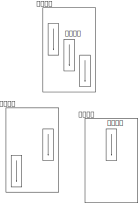
\includegraphics[width=\textwidth]{out/pdf/svg/process_threads.pdf}
    \end{column}    
  \end{columns}
\ao{プロセス $=$ アドレス空間(箱) $+$ 1つ以上のスレッド}
\end{frame}

%%%%%%%%%%%%%%%%% 
\begin{frame}
  \frametitle{用語の注: CPU, コア, プロセッサ, \ldots}
  \begin{columns}
    \begin{column}{0.65\textwidth}
      \begin{itemize}
      \item \ao{CPU} $\supset$ \ao{物理コア} $\supset$ \ao{仮想コア} 
        \begin{itemize}
        \item<1-> 1 \ao{CPU} に複数(2〜64程度)の\ao{物理コア}
          \ao{(マルチコアCPU)}
        \item<2-> 1 \ao{物理コア} に複数(2〜8程度)の\ao{仮想コア}
          (Simultaneous Multithreading \ao{(SMT)},
          ハイパースレッディング(Intel用語))
        \end{itemize}
      \end{itemize}
    \end{column}
    \begin{column}{0.35\textwidth}
      \begin{center}
        \includegraphics[width=\textwidth]{out/pdf/svg/cpu.pdf}
      \end{center}
    \end{column}
  \end{columns}
  \begin{itemize}
  \item<3->
    各 \ao{仮想コア} $=$ 「命令の取り出し, 実行」を実行するハードの機能
  \item<4-> つまり仮想コア数分までのスレッドは「ほんとに同時に」実行される
  \item<5-> スレッドに
    \mura{「CPUを割り当てる」}と言うが実際に割り当てているのは,
    1つの仮想コア
  \end{itemize}
\end{frame}

%%%%%%%%%%%%%%%%% 
\begin{frame}
  \frametitle{ややこしい注}
\begin{itemize}
\item 物理コア vs. 仮想コア
  \begin{itemize}
  \item 性能を気にしなければ,
    仮想コアと物理コアの違いを意識する場面はほぼ無い
  \item 1物理コア中の仮想コアは\ao{演算器を共有}
  \item $\Rightarrow$1物理コアに複数のスレッドを同時に走らせても,
    (1つのスレッドだけですでに性能を出し尽くしている場合)
    性能が向上しない場合がある
  \end{itemize}
  
\item \ao{OSが見せるプロセッサ数は, 普通, 仮想コア数}
  \begin{itemize}
  \item Linux : {\tt cat /proc/cpuinfo}, システムモニタ
  \item Windows : タスクマネージャ, リソースモニタ
  \end{itemize}
\item \ao{仮想コア} $=$ \ao{ハードウェアスレッド} (同義語)
\item \ao{プロセッサ}は曖昧な言葉
  \begin{itemize}
  \item CPU, 物理コア, 仮想コアなどの意味で使われる
  \end{itemize}
\item 単に\ao{コア}ということもしばしば; 物理コア, 仮想コアのどちらを
  意味するか曖昧
\end{itemize}
\end{frame}

%%%%%%%%%%%%%%%%% 
\begin{frame}
\frametitle{スレッドを観察するコマンド}
\begin{itemize}
\item Unix CUI
  \begin{itemize}
  \item \ao{\tt ps auxmww}
  \item \ao{\tt top -H} (HでToggle)
  \end{itemize}
\item Linux
  \begin{itemize}
  \item \ao{\tt /proc/{\it pid}/task/{\it tid}}
  \end{itemize}
\end{itemize}
\end{frame}

%%%%%%%%%%%%%%%%% 
\begin{frame}
\frametitle{Unix: スレッド関連のAPI}
\begin{itemize}
\item \ao{POSIXスレッド} (または単に{\tt Pthreads})
  \begin{itemize}
  \item POSIX : Portable Operating System Interface (Unix系OS共通のAPI仕様)
  \end{itemize}
\item \ao{\tt pthread\_create}
  \begin{itemize}
  \item スレッドを作る
  \end{itemize}
\item \ao{\tt pthread\_exit}
  \begin{itemize}
  \item 現スレッドを終了
  \end{itemize}
\item \ao{\tt pthread\_join}
  \begin{itemize}
  \item スレッドの終了を待つ
  \end{itemize}
\item その他多数(後の週)
\end{itemize}
\end{frame}
  
%%%%%%%%%%%%%%%%% 
\begin{frame}
\frametitle{スレッドの生成〜終了〜処理}
\begin{columns}
  \begin{column}{0.5\textwidth}
    \begin{enumerate}
    \item<2-> {\tt pthread\_create}により子スレッドが生成される
    \item<4-> 子スレッドが終了する({\tt pthread\_exit}を呼ぶ,
      または子スレッド生成時に指定した関数が終了)
    \item<6-> どれかのスレッドが{\tt pthread\_join}を呼ぶ
    \end{enumerate}
  \end{column}
  \begin{column}{0.5\textwidth}
\begin{center}
\only<1>{\includegraphics[height=0.7\textheight]{out/pdf/svg/thread_1.pdf}}%
\only<2>{\includegraphics[height=0.7\textheight]{out/pdf/svg/thread_2.pdf}}%
\only<3>{\includegraphics[height=0.7\textheight]{out/pdf/svg/thread_3.pdf}}%
\only<4>{\includegraphics[height=0.7\textheight]{out/pdf/svg/thread_4.pdf}}%
\only<5>{\includegraphics[height=0.7\textheight]{out/pdf/svg/thread_5.pdf}}%
\only<6>{\includegraphics[height=0.7\textheight]{out/pdf/svg/thread_6.pdf}}%
\end{center}
  \end{column}
\end{columns}
\end{frame}

%%%%%%%%%%%%%%%%% 
\begin{frame}[fragile]
\frametitle{{\tt pthread\_create}}
\begin{itemize}
\item {\tt pthread\_create({\it tid}, {\it attr}, {\it f}, {\it arg})}
\item {\tt {\it f}({\it arg})}を実行するスレッド(子スレッド)を作る
  $\equiv$ {\tt pthread\_create}呼び出し以降と,
  {\tt {\it f}({\it arg})}が並行して実行される
\item $f$は{\tt void*}を受け取り{\tt void*}を返す関数
\item スレッドの\ao{開始関数}と呼ぶ(あまり一般的でない用語)
\item 諸々の属性を{\tt {\it attr}}で指定(manを見よ)
\item {\tt pthread\_create}のreturn後,
  子スレッドのIDが{\tt *{\it tid}}に書き込まれる
\end{itemize}
\end{frame}

%%%%%%%%%%%%%%%%% 
\begin{frame}[fragile]
\frametitle{{\tt pthread\_exit({\it p})}}
\begin{itemize}
\item {\tt pthread\_exit}を呼んだプロセスを,
  指定した終了ステータス{\it p}で終了させる
\item {\it p} : ポインタ({\tt void *})
\item スレッドの開始関数が終了した場合も同じ効果
  \begin{itemize}
  \item 開始関数の返り値(return value)が終了ステータス
  \end{itemize}
\item {\it p}は{\tt pthread\_join}で取得可能
\end{itemize}
\end{frame}

%%%%%%%%%%%%%%%%% 
\begin{frame}[fragile]
  \frametitle{{\tt pthread\_join}}
  \begin{itemize}
  \item {\tt pthread\_join({\it tid}, {\it q})}
  \item 子スレッド{\it tid}の終了を待つ
  \item {\it tid}の終了ステータスが{\tt *{\it q}}に返される
  \item {\tt waitpid}のスレッド版だが細かい違い:
    \begin{itemize}
    \item {\tt pthread\_join({\it tid}, {\it q})}を呼ぶのは,
      {\it tid}の親スレッドである必要はない(同じプロセス中のどのスレッドでもよい)
    \end{itemize}
  \end{itemize}
\end{frame}

%%%%%%%%%%%%%%%%% 
\begin{frame}
  \frametitle{プロセス vs. スレッド}
  \begin{columns}
    \begin{column}{0.7\textwidth}
      \begin{itemize}
      \item 同じプロセス内の\ao{スレッドは「アドレス空間」を共有}する
        \begin{itemize}
        \item $\approx$プログラム内のデータを共有する
        \item $\approx$あるスレッドが書き込んだ値は他のスレッドも自動的に観測する
        \end{itemize}
      \item 複数の\ao{プロセスはそれぞれ独立した「アドレス空間」}を持つ
        \begin{itemize}
        \item $\approx$プログラム内のデータは共有されない
        \item $\approx$あるプロセスが書き込んだ値が他のプロセスに観測されることはない
          (その仕組みおよび例外は後の週で)
        \end{itemize}
      \end{itemize}
    \end{column}
    \begin{column}{0.3\textwidth}
      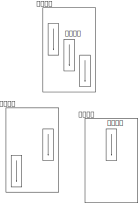
\includegraphics[width=\textwidth]{out/pdf/svg/process_threads.pdf}
    \end{column}
  \end{columns}
\end{frame}

  
\end{document}
